
\documentclass[10pt]{beamer}
\usetheme{umbc2}
\useinnertheme{umbcboxes}
\setbeamercolor{umbcboxes}{bg=violet!12,fg=black}

\usepackage{longtable}
\usepackage{tabu}
\usepackage{subeqnar}

\newcommand{\ul}{\underline}
\newcommand{\be}{\begin{equation}}
\newcommand{\ee}{\end{equation}}
\newcommand{\bdm}{\begin{displaymath}}
\newcommand{\edm}{\end{displaymath}}
\newcommand{\bea}{\begin{eqnarray}}
\newcommand{\eea}{\end{eqnarray}}
\newcommand{\bsea}{\begin{subeqnarray*}}
\newcommand{\esea}{\end{subeqnarray*}}
\newcommand{\mb}[1]{\mbox{#1}}
\newcommand{\mc}[3]{\multicolumn{#1}{#2}{#3}}
\newcommand{\bm}[1]{\mbox{\bf #1}}
\newcommand{\bmm}[1]{\mbox{\boldmath$#1$\unboldmath}}
\newcommand{\bmell}{\bmm\ell}
\newcommand{\hateps}{\widehat{\bmm\varepsilon}}
\newcommand{\graybox}[1]{\psboxit{box .9 setgray fill}{\fbox{#1}}}
\newcommand{\mdeg}[1]{\mbox{$#1^{\mbox{\scriptsize o}}$}}
\newcommand{\dd}{\mbox{\footnotesize{$\nabla \! \Delta$}}}
\newcommand{\p}{\partial\,}
\renewcommand{\d}{\mbox{d}}
\newcommand{\dspfrac}{\displaystyle\frac}
\newcommand{\nl}{\\[4mm]}

\title{Processing GNSS Data in Real-Time}

\author{Leo\v{s} Mervart}

\institute{TU Prague}

\date{Frankfurt, January 2014}

% \AtBeginSection[]
% {
%   \begin{frame}
%     \frametitle{Table of Contents}
%     \tableofcontents[currentsection]
%   \end{frame}
% }

\begin{document}

%%%%%%%%%%%%%%%%%%%%%%%%%%%%%%%%%%%%%%%%%%%%%%%%%%%%%%%%%%%%%%%%%%%%%%%%%%%%%%%%

\begin{frame}
  \titlepage
\end{frame}

%%%%%%%%%%%%%%%%%%%%%%%%%%%%%%%%%%%%%%%%%%%%%%%%%%%%%%%%%%%%%%%%%%%%%%%%%%%%%%%%

\begin{frame}
\frametitle{Medieval Times of GNSS (personal memories)}

\begin{description}
\item[1991] Prof. Gerhard Beutler became the director of the Astronomical Institute, University of
  Berne. The so-called Bernese GPS Software started to be used for (post-processing) analyzes of
  GNSS data.
\item[1992] LM started his PhD study at AIUB.
\item[1992] Center for Orbit Determination in Europe (consortium of AIUB, Swisstopo, BKG, IGN, and
  IAPG/TUM) established. Roughly at that time LM met Dr. Georg Weber for the first time.
\item[1993] International GPS Service formally recognized by the IAG.
\item[1994] IGS began providing GPS orbits and other products routinely (January, 1).
\item[1995] GPS declared fully operational.
\end{description}

\end{frame}

%%%%%%%%%%%%%%%%%%%%%%%%%%%%%%%%%%%%%%%%%%%%%%%%%%%%%%%%%%%%%%%%%%%%%%%%%%%%%%%%

\begin{frame}
\frametitle{CODE-Related Works in 1990's}

\begin{itemize}
\item The Bernese GPS Software was the primary tool for CODE analyzes (Fortran~77).
\item IGS reference network was sparse.
\item Real-time data transmission limited (Internet was still young, TCP/IP widely accepted 1989).
\item CPU power of then computers was limited (VAX/VMS OS used at AIUB).
\end{itemize}

In 1990's high precision GPS analyzes were almost exclusively performed in post-processing mode.
The typical precise application of GPS at that time was the processing of a network of static
GPS-only receivers for the estimation of station coordinates.

\end{frame}

%%%%%%%%%%%%%%%%%%%%%%%%%%%%%%%%%%%%%%%%%%%%%%%%%%%%%%%%%%%%%%%%%%%%%%%%%%%%%%%%

\begin{frame}
\frametitle{Tempora mutantur (and maybe ``nos mutamur in illis'')}

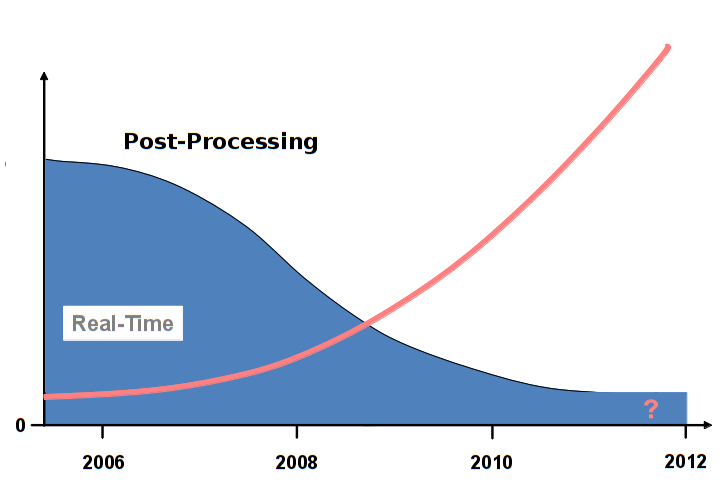
\includegraphics[width=0.7\textwidth,angle=0]{pp_vs_rt.png}

\vspace*{-2cm}
\hspace*{6cm}
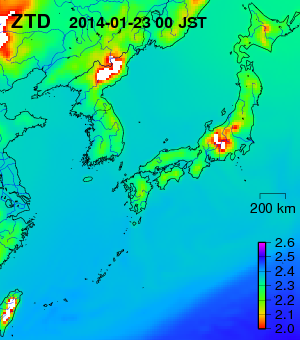
\includegraphics[width=0.4\textwidth,angle=0]{ea_ztd_21h.png}


\end{frame}


%%%%%%%%%%%%%%%%%%%%%%%%%%%%%%%%%%%%%%%%%%%%%%%%%%%%%%%%%%%%%%%%%%%%%%%%%%%%%%%%

\begin{frame}
\frametitle{O tempora! O mores!}

\begin{itemize}
\item people want more and more \ldots
\item everybody wants everything immediately \ldots
\item \hspace*{2cm} and, of course, free of charge \ldots
\end{itemize}
\vspace*{5mm}
In GNSS-world it means:
\begin{itemize}
\item There are many new kinds of GNSS applications - positioning is becoming just one of many
  purposes of GNSS usage.
\item Many results of GNSS processing are required in real-time (or, at least, with very small
  delay).
\item GPS is not the only positioning system. Other GNSS are being established (for practical but
  also for political reasons).
\item People are used that many GNSS services are available free of charge (but the development and
  maintenance has to be funded). 
\end{itemize}

\begin{block}{But \ldots}
\end{block}

\end{frame}

%%%%%%%%%%%%%%%%%%%%%%%%%%%%%%%%%%%%%%%%%%%%%%%%%%%%%%%%%%%%%%%%%%%%%%%%%%%%%%%%

\begin{frame}
\frametitle{Nihil novi sub sole}

Each GNSS-application is based on processing code and/or phase observations
\vspace*{-3mm}
  \begin{eqnarray*}
  P^i & = & \varrho^i + c\;\delta - c\;\delta^i + T^i + I^i + b_P              \\
  L^i & = & \varrho^i + c\;\delta - c\;\delta^i + T^i - I^i + b^i
  \end{eqnarray*}
  where
  \begin{tabbing}
  $P^i$, $L^i$ ~~~~~~~ \= are the code and phase measurements, \\ 
  $\varrho^i$          \> is the travel distance between the satellite 
                          and the receiver,                               \\
  $\delta$, $\delta^i$ \> are the receiver and satellite clock errors,    \\
  $I^i$                \> is the ionospheric delay,                       \\
  $T^i$                \> is the tropospheric delay,                      \\
  $b_P$                \> is the code bias, and                           \\
  $b^i$                \> is the phase bias (including initial
                          phase ambiguity).
  \end{tabbing}
Observation equations reveal what information can be gained from processing GNSS data:
\begin{itemize}
\item geometry (receiver positions, satellite orbits), and
\item state of atmosphere (both dispersive and non-dispersive part)
\end{itemize}
The observation equations also show that, in principle, GNSS is an
\textcolor{blue!90}{interferometric} technique -- precise results are actually always relative.

\end{frame}

%%%%%%%%%%%%%%%%%%%%%%%%%%%%%%%%%%%%%%%%%%%%%%%%%%%%%%%%%%%%%%%%%%%%%%%%%%%%%%%%

\begin{frame}
\frametitle{Challenges of Real-Time GNSS Application}
\begin{itemize}
\item Suitable algorithms for the parameter adjustment have to be used (filter techniques instead
  of classical least-squares).
\item Reliable data links have to been established (between rover station and a reference station,
  between receivers and processing center, or between processing center and DGPS correction
  provider).
\item Software tools for handling real-time data (Fortran is not the best language for that).
\item Fast CPUs.
\end{itemize}

As said above -- GNSS is an interferometric technique. Processing of a single station cannot give
precise results. However, data of reference station(s) can be replaced by the so-called corrections
(DGPS corrections, precise-point positioning etc.) These techniques are particularly suited for
real-time applications because the amount of data being transferred can be considerably reduced.

\end{frame}

%%%%%%%%%%%%%%%%%%%%%%%%%%%%%%%%%%%%%%%%%%%%%%%%%%%%%%%%%%%%%%%%%%%%%%%%%%%%%%%%

\begin{frame}
\frametitle{Algorithms -- Kalman Filter}

\begin{small}

State vectors $\bmm{x}$ at two subsequent epochs are
related to each other by the following linear equation:
\bdm
\bmm{x}(n) = \bmm{\Phi}\; \bmm{x}(n-1) + \bmm{\Gamma}\;\bmm{w}(n)~,
\edm
where $\Phi$ and $\Gamma$ are known matrices and {\em white noise} $\bmm{w}(n)$ is a random
vector with the following statistical properties:
\bsea
E(\bmm{w})                  & = & \bmm{0}                           \\
E(\bmm{w}(n)\;\bmm{w}^T(m)) & = & \bmm{0} ~~ \mbox{for $m \neq n$}  \\
E(\bmm{w}(n)\;\bmm{w^T}(n)) & = & \bm{Q}_s(n) ~.
\esea

Observations $\bmm{l}(n)$ and the state vector $\bmm{x}(n)$ are related to
each other by the linearized {\em observation equations} of form
\bdm \label{eq:KF:obseqn}
 \bmm{l}(n) = \bm{A}\;\bmm{x}(n) + \bmm{v}(n) ~ ,
\edm
where $\bm{A}$ is a known matrix (the so-called {\em first-design matrix}) and
$\bmm{v}(n)$ is a vector of random errors with the following properties:
\bsea\label{eq:KF:resid}
E(\bmm{v})                  & = & \bmm{0} \\
E(\bmm{v}(n)\;\bmm{v}^T(m)) & = & \bmm{0} ~~ \mbox{for $m \neq n$}  \\
E(\bmm{v}(n)\;\bmm{v^T}(n)) & = & \bm{Q}_l(n) ~.
\esea

\end{small}

\end{frame}

%%%%%%%%%%%%%%%%%%%%%%%%%%%%%%%%%%%%%%%%%%%%%%%%%%%%%%%%%%%%%%%%%%%%%%%%%%%%%%%%

\begin{frame}
\frametitle{Classical KF Form}

Minimum Mean Square Error (MMSE) estimate $\widehat{\bmm{x}}(n)$ of vector
$\bmm{x}(n)$ meets the condition
$E\left((\bmm{x} - \widehat{\bmm{x}})(\bmm{x} - \widehat{\bmm{x}})^T\right) =
\mbox{min}$ and is given by
\begin{subeqnarray}\label{eq:KF:prediction}
 \widehat{\bmm{x}}^-(n) & = & \bmm{\Phi} \widehat{\bmm{x}}(n-1)         \\
 \bm{Q}^-(n)            & = & \bmm{\Phi} \bm{Q}(n-1) \bmm{\Phi}^T + 
                          \bmm{\Gamma} \bm{Q}_s(n) \bmm{\Gamma}^T   
\end{subeqnarray}
\begin{subeqnarray}\label{eq:KF:update}
 \widehat{\bmm{x}}(n)   & = & \widehat{\bmm{x}}^-(n) + 
                              \bm{K}\left(\bmm{l} - 
                              \bm{A}\widehat{\bmm{x}}(n-1)\right) \\
 \bm{Q}(n)              & = & \bm{Q}^-(n) - \bm{K}\bm{A}\bm{Q}^-(n) ~,
\end{subeqnarray}
where
\bdm \label{eq:KF:KandH}
 \bm{K} = \bm{Q}^-(n)\bm{A}^T\bm{H}^{-1}, \quad
 \bm{H} = \bm{Q}_l(n) + \bm{A}\bm{Q}^-(n)\bm{A}^T ~.
\edm
Equations (\ref{eq:KF:prediction}) are called {\em prediction}, 
equations (\ref{eq:KF:update}) are called {\em update} step of Kalman filter.

\end{frame}

%%%%%%%%%%%%%%%%%%%%%%%%%%%%%%%%%%%%%%%%%%%%%%%%%%%%%%%%%%%%%%%%%%%%%%%%%%%%%%%%

\begin{frame}
\frametitle{Square-Root Filter} \label{sec:SRF}
\begin{small}
Algorithms based on equations (\ref{eq:KF:prediction}) and
(\ref{eq:KF:update}) may suffer from numerical instabilities that are primarily
caused by the subtraction in (\ref{eq:KF:update}b). This deficiency may be
overcome by the so-called {\em square-root} formulation of the Kalman filter
that is based on the so-called {\em QR-Decomposition}. Assuming the 
Cholesky decompositions
\be \label{eq:SRF:defsym}
  \bm{Q}(n)   = \bm{S}^{T} \bm{S}  , \quad
  \bm{Q}_l(n) = \bm{S}^T_l \bm{S}_l,  \quad
  \bm{Q}^-(n) = \bm{S}^{-T}\bm{S}^- 
\ee
we can create the following block matrix and its QR-Decomposition:
\be \label{eq:SRF:main}
 \left(\begin{array}{ll} 
   \bm{S}_l         & \bm{0} \\
  \bm{S}^-\bm{A}^T  & \bm{S}^-
 \end{array}\right)
=
 N \left(\begin{array}{cc} 
    \bm{X}     & \bm{Y} \\
    \bm{0}     & \bm{Z}
   \end{array}\right) ~ .
\ee
It can be easily verified that 
\bsea\label{eq:SRF:HK}
 \bm{H}    & = & \bm{X}^T\bm{X}   \\
 \bm{K}^T  & = & \bm{X}^{-1}\bm{Y}\\
 \bm{S}    & = & \bm{Z}           \\
 \bm{Q}(n) & = & \bm{Z}^T\bm{Z} ~ .
\esea
State vector $\widehat{\bmm{x}}(n)$ is computed in a usual way using the
equation (\ref{eq:KF:update}a).
\end{small}
\end{frame}

%%%%%%%%%%%%%%%%%%%%%%%%%%%%%%%%%%%%%%%%%%%%%%%%%%%%%%%%%%%%%%%%%%%%%%%%%%%%%%%%

\begin{frame}
\frametitle{Data Transfer -- NTRIP}

In order to be useful data have to be provided in a well-defined \textcolor{blue}{format}.
RTCM (Radio Technical Commission for Maritime Services) messages are widely used for GNSS data in
real-time. 

\vspace*{5mm}

In addition to a format the so-called \textcolor{blue}{protocol} has to be defined. Using a given
protocol the data user communicates with the data provider.

For GNSS data, the so-called \textcolor{blue}{NTRIP} streaming protocol is used.
\begin{itemize}
\item NTRIP stands for Networked Transport of RTCM via Internet Protocol.
\item NTRIP is in principle a layer on top of TCP/IP.
\item NTRIP has been developed at BKG (together with TU Dortmund).
\item NTRIP is capable of handling hundreds of data streams simultaneously delivering the data
to thousands of users.
\item NTRIP is world-wide accepted.
\end{itemize}

\end{frame}

%%%%%%%%%%%%%%%%%%%%%%%%%%%%%%%%%%%%%%%%%%%%%%%%%%%%%%%%%%%%%%%%%%%%%%%%%%%%%%%%

\begin{frame}
\frametitle{NTRIP}

Efficiency of data transfer using NTRIP is achieved thanks to the GNSS Internet Radio /
IP-Streaming architecture:

\begin{center}
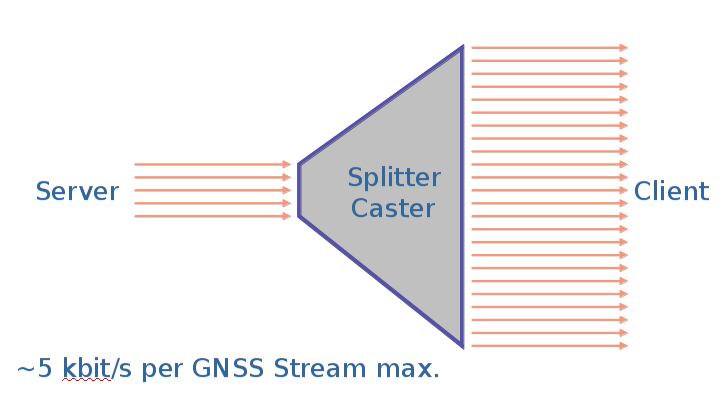
\includegraphics[width=0.7\textwidth,angle=0]{ntrip.png}
\end{center}

\end{frame}

%%%%%%%%%%%%%%%%%%%%%%%%%%%%%%%%%%%%%%%%%%%%%%%%%%%%%%%%%%%%%%%%%%%%%%%%%%%%%%%%

\begin{frame}
\frametitle{BKG Ntrip Client (BNC)}

An important reason why NTRIP has been widely accepted is that BKG provided high-quality public
license software tools for its usage. One of these tools is the so-called \textcolor{blue}{BKG
Ntrip Client}.

  \begin{itemize}
  \item BNC source consists currently of approximately 50.000 lines of code 
  \item approximately 90 \% is C++, 10 \% standard C
  \item BNC uses a few third-party pieces of software (first of all the RTCM
    decoders/encoders and a matrix algebra library)
  \end{itemize}

  \begin{block}{BNC is intended to be}
  \begin{itemize}
  \item user-friendly
  \item cross-platform
  \item easily modifiable (by students, GNSS beginners)
  \item useful (at least a little bit ...)
  \end{itemize}
  \end{block}

  \begin{block}{BNC is not only an NTRIP client \ldots}
  \end{block}

\end{frame}

%%%%%%%%%%%%%%%%%%%%%%%%%%%%%%%%%%%%%%%%%%%%%%%%%%%%%%%%%%%%%%%%%%%%%%%%%%%%%%%%

\begin{frame}
  \frametitle{Data QC in BNC}
  \begin{center}
    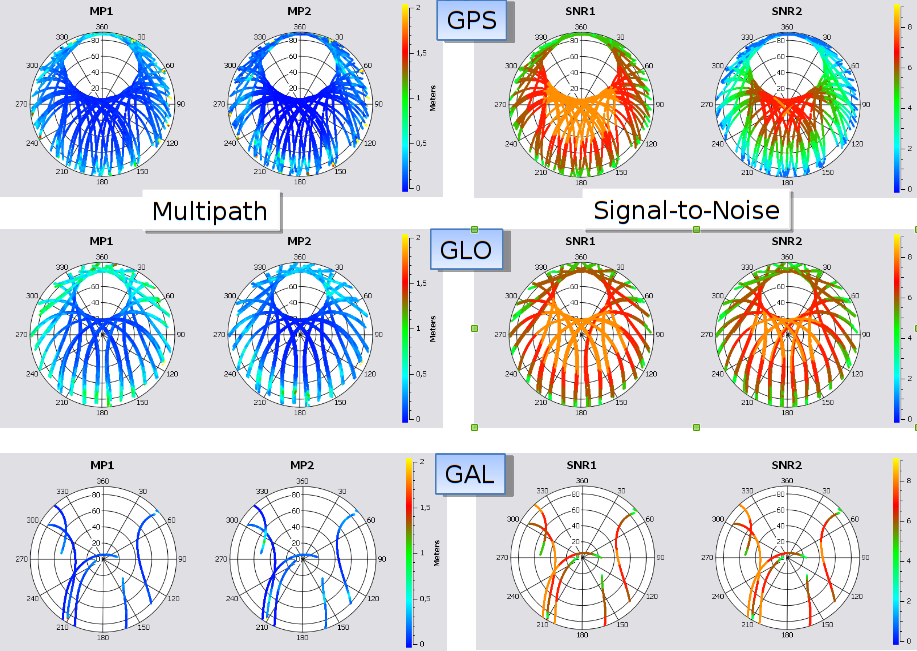
\includegraphics[width=0.9\textwidth,angle=0]{bnc_qc1.png}
  \end{center}
\end {frame}

%%%%%%%%%%%%%%%%%%%%%%%%%%%%%%%%%%%%%%%%%%%%%%%%%%%%%%%%%%%%%%%%%%%%%%%%%%%%%%%%

\begin{frame}
  \frametitle{Precise Point Positioning with PPP}
  \begin{center}
    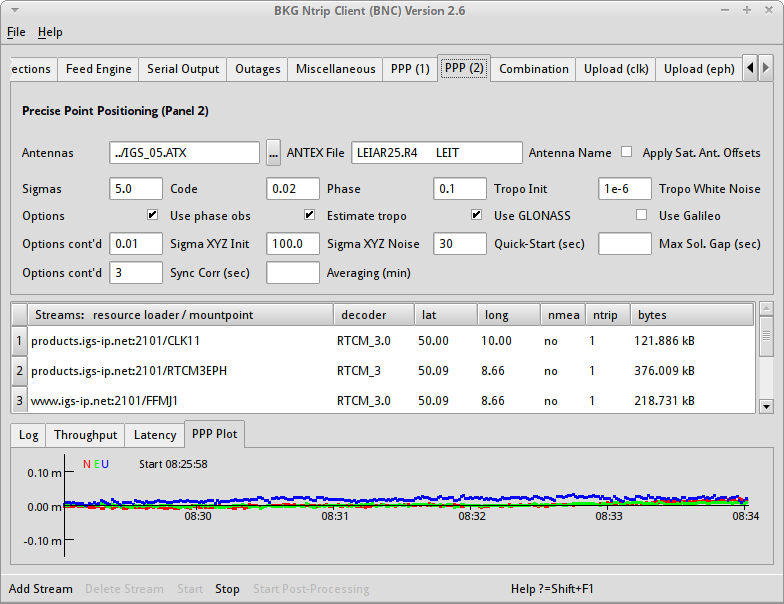
\includegraphics[width=0.9\textwidth,angle=0]{ppp1.png}
  \end{center}
\end {frame}

%%%%%%%%%%%%%%%%%%%%%%%%%%%%%%%%%%%%%%%%%%%%%%%%%%%%%%%%%%%%%%%%%%%%%%%%%%%%%%%%

\begin{frame}
  \frametitle{Precise Point Positioning with PPP (cont.)}
  BNC provides a good framework for the PPP client (observations, orbits, and
  corrections stand for disposal). 

  Main reasons for the PPP module in BNC have been:
  \begin{itemize}
  \item monitoring the quality of incoming data streams (primarily the PPP
    corrections) 
  \item providing a simple easy-to-use tool for the basic PPP positioning 
  \end{itemize}

  The PPP facility in BNC is provided in the hope that it will be useful.
  \begin{itemize}
  \item The mathematical model of observations and the adjustment algorithm are
    implemented in such a way that they are (according to our best knowledge)
    correct without any shortcomings, however,
  \item we have preferred simplicity to transcendence, and
  \item the list of options the BNC users can select is limited.
  \item[$\Rightarrow$] Commercial PPP clients may outperform BNC in some
    aspects.
  \end{itemize}
  We believe in a possible good coexistence of the commercial software and
  open source software.
\end {frame}

%%%%%%%%%%%%%%%%%%%%%%%%%%%%%%%%%%%%%%%%%%%%%%%%%%%%%%%%%%%%%%%%%%%%%%%%%%%%%%%%

\begin{frame}
  \frametitle{PPP Options}
  \begin{itemize}
  \item single station, SPP or PPP
  \item real-time or post-processing
  \item processing of code and phase ionosphere-free combinations, GPS,
    Glonass, and Galileo
  \end{itemize}
  \begin{center}
    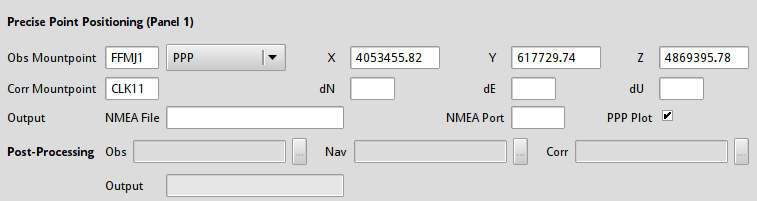
\includegraphics[width=0.9\textwidth,angle=0]{ppp_opt1.png} \\[2mm]
    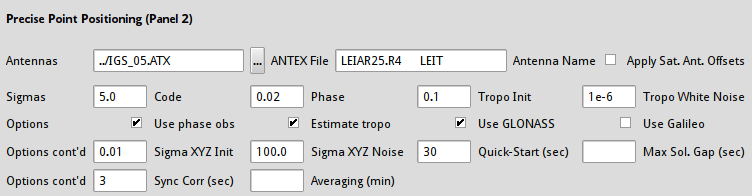
\includegraphics[width=0.9\textwidth,angle=0]{ppp_opt2.png}
  \end{center}
\end {frame}


\end{document}
